\documentclass[12pt]{article}
\usepackage[english]{babel}
\usepackage[utf8x]{inputenc}
\usepackage{amsmath}
\usepackage{subfigure, float}
\usepackage{graphicx, lipsum,caption}
\usepackage[colorinlistoftodos]{todonotes}

\begin{document}
	
	\begin{titlepage}
		
		\newcommand{\HRule}{\rule{\linewidth}{0.5mm}} % Defines a new command for the horizontal lines, change thickness here
		
		\center % Center everything on the page
		
		%----------------------------------------------------------------------------------------
		%	HEADING SECTIONS
		%----------------------------------------------------------------------------------------
		
		\textsc{\LARGE Central Washington University}\\[1.5cm] % Name of your university/college
		\textsc{\Large Advanced Algorithms}\\[0.5cm] % Major heading such as course name
		\textsc{\large Winter 2019}\\[0.5cm] % Minor heading such as course title
		
		%----------------------------------------------------------------------------------------
		%	TITLE SECTION
		%----------------------------------------------------------------------------------------
		
		\HRule \\[0.4cm]
		{ \huge \bfseries Project 5 Report}\\[0.4cm] % Title of your document
		\HRule \\[1.5cm]
		
		%----------------------------------------------------------------------------------------
		%	AUTHOR SECTION
		%----------------------------------------------------------------------------------------
		
		\begin{minipage}{0.4\textwidth}
			\begin{flushleft} \large
				\emph{Author:}\\
				Hermann \textsc{Yepdjio} % Your name
			\end{flushleft}
		\end{minipage}
		~
		\begin{minipage}{0.4\textwidth}
			\begin{flushright} \large
				\emph{Professor:} \\
				Dr. Razvan \textsc{Andonie} % Supervisor's Name
			\end{flushright}
		\end{minipage}\\[1cm]
		
		% If you don't want a supervisor, uncomment the two lines below and remove the section above
		%\Large \emph{Author:}\\
		%John \textsc{Smith}\\[3cm] % Your name
		
		%----------------------------------------------------------------------------------------
		%	DATE SECTION
		%----------------------------------------------------------------------------------------
		
		{\large \today}\\ % Date, change the \today to a set date if you want to be precise
		
		%----------------------------------------------------------------------------------------
		%	LOGO SECTION
		%----------------------------------------------------------------------------------------
		
		
\includegraphics[width=12cm]{CWU-Logo.png}\\[.5cm] % Include a department/university logo - this will require the graphicx package
		
		%----------------------------------------------------------------------------------------
		
		\vfill % Fill the rest of the page with whitespace
		
	\end{titlepage}
	\newpage
	\tableofcontents
	\newpage
	
	
	
	\section{Introduction}
		The Aho-Corasick string matching algorithm is a fast and memory efficient algorithm invented by Alfred V. Aho and Margaret J. Corasick. Given a list of patterns to find in a given input text, the algorithm will locate all the occurrences of the patterns in the input text by matching them all at once instead of one at the time. The goal of this project was to implement in python both the Aho-Corasick algorithm and a naive approach (which matches the patterns one at the time using the python's string.find() function) and compare both implementations by running some experiments.
	
	\section{implementation}
		We implemented both algorithms so that they will find only the last occurrence of the patterns instead of finding all the occurrences. When a pattern is found, a message containing the pattern itself and information about its position in the text input, is printed on the screen. 
		\subsection{Naive String Matching Approach}
			\begin{itemize}
				\item The algorithm takes as input the name of the input text file and the list of patterns to look for,
				\item the text file is open and its whole content is read as a single string, 
				\item the algorithm loops over the list of patterns calling the string.rfind() function on the text input with the current pattern as parameter at each iteration. The string.rfind(x) function is another version of string.find(x) which looks for the last occurrence of a in string instead of the first occurrence.
			\end{itemize}
		
		\subsection{Aho-Corasick String Matching Approach}
			This algorithm uses the pyahocorasick package. 
			\begin{itemize}
				\item The algorithm takes as input the name of the input text file and the list of patterns to look for,
				\item the text file is open and its whole content is read as a single string,
				\item an empty automaton is created using the pyahochorasick package and populated with every single word in the input text
				\item the algorithm loops over the list of patterns calling the automaton.get(pattern) function at each iteration, in order to find the last occurrence of the current pattern in the text input.
			\end{itemize}
			  
		
	\section {experimentation process}
		For the experimentation, we ran the algorithm using 10 files (for input text) of different sizes ( ranging from 12324 to 5182632 words) and 7 other files (for patterns) of different sizes (ranging from 20 to 4941 words). We recorded the time taken for each algorithm to string match each pattern list to all the input text and the results are shown and discussed in the next section. 
	
	\section{Results}
		\subsection{Rlots for running time }
			
			The figures below show the results we got during the experimentation process. 
			\begin{itemize}
				\item The green curve represents the Aho-Corasick implementation
				\item The red curve represents the naive string matching implementation. 
			\end{itemize}
			\begin{figure}[H]
				\subfigure[number of pattern: 20]{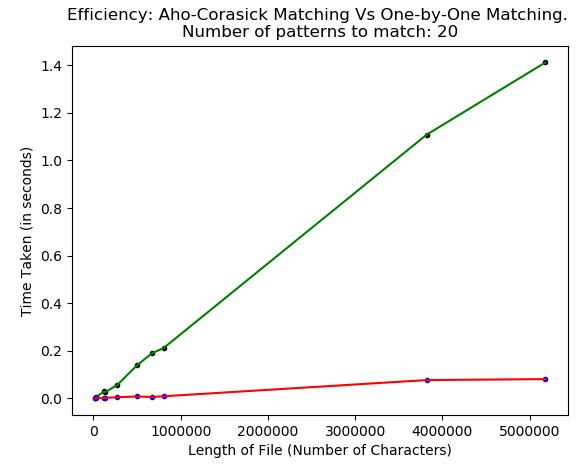
\includegraphics[width=6cm]{pattern_size_20.PNG}}
				\hfill
				\subfigure[number of patterns: 179]{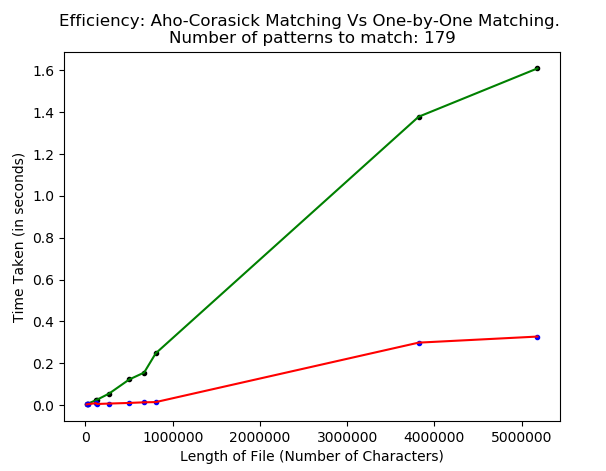
\includegraphics[width=6cm]{pattern_size_179.PNG}}
				\hfill
			\end{figure}
			\begin{figure}[H]
				\subfigure[number of patterns: 504]{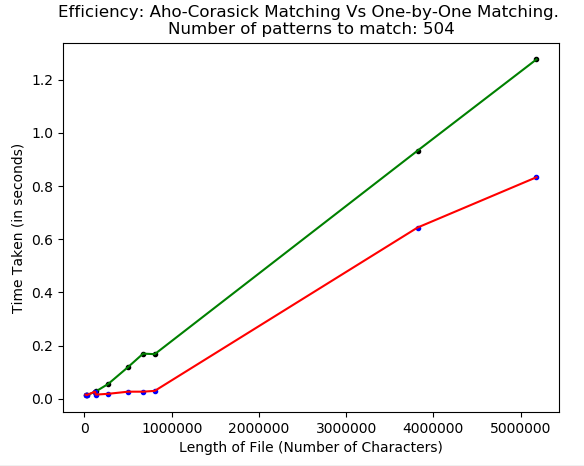
\includegraphics[width=6cm]{pattern_size_504.PNG}}
				\hfill
				\subfigure[number of patterns: 2240]{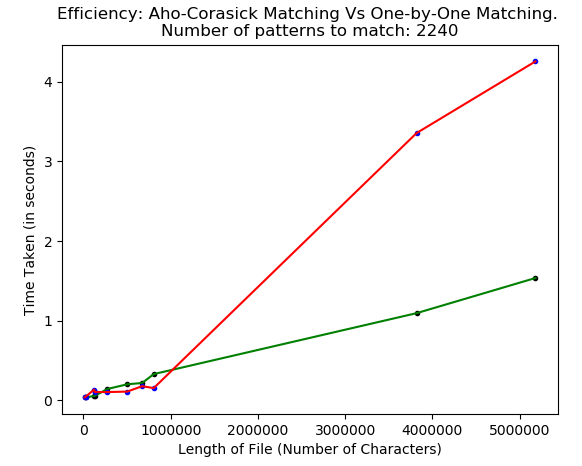
\includegraphics[width=6cm]{pattern_size_2240.PNG}}
				\hfill
			\end{figure}
			\begin{figure}[H]
				\subfigure[number of patterns: 3269]{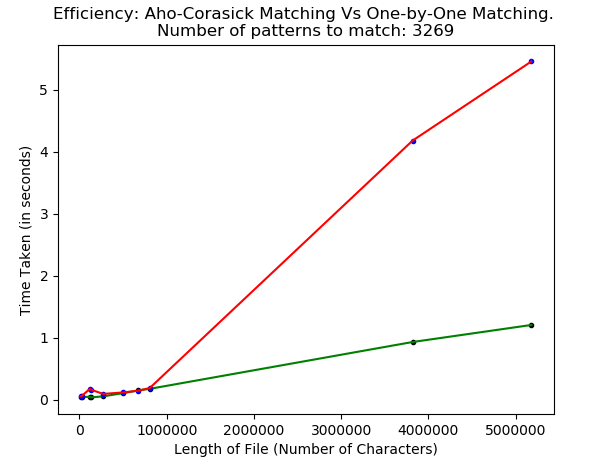
\includegraphics[width=6cm]{pattern_size_3269.PNG}}
				\hfill
				\subfigure[number of patterns: 4032]{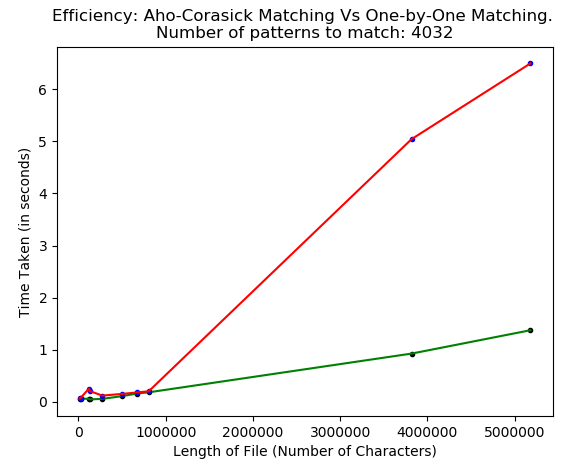
\includegraphics[width=6cm]{pattern_size_4032.PNG}}
				\hfill
			\end{figure}
		\begin{center}
				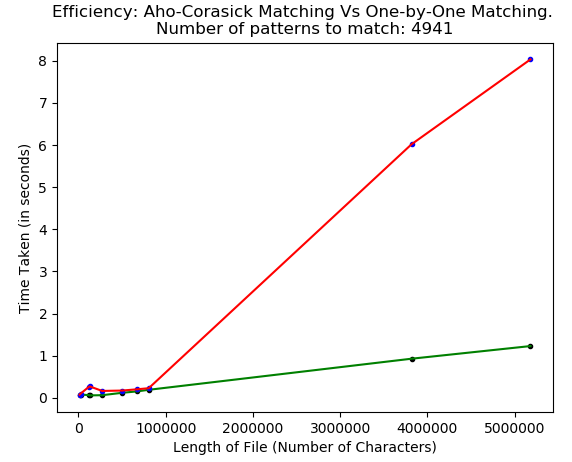
\includegraphics[width=6cm]{pattern_size_4941.PNG}\\
				(g) number of patterns: 4941
			\hfill
		\end{center}
	
		\subsection{Observation}
			As we can see from figures a, b and c above, the naive approach (red curve) is faster than Aho-Corasick (green curve) for small numbers of patterns ($n \leq 54$ in our case). figures d through g show that as the number of patterns increases the Aho-Corasick algorithm becomes way faster than the naive approach. 
		
			
	\section{Conclusion}
		After experimenting with the naive string matching approach and the Aho-Corasick implementation, we can conclude that when the number of patterns to be matched is relatively small, it is better to use the naive string matching implementation and when the number of patterns to be matched is relatively big, then it is better to use the Aho-Corasick implementation. 
		
	
\end{document}
